\documentclass[12pt,english]{article}
\usepackage{mathptmx}

\usepackage{color}
\usepackage[dvipsnames]{xcolor}
\definecolor{darkblue}{RGB}{0.,0.,139.}

\usepackage[top=1in, bottom=1in, left=1in, right=1in]{geometry}

\usepackage{amsmath}
\usepackage{amstext}
\usepackage{amssymb}
\usepackage{setspace}
\usepackage{lipsum}

\usepackage[authoryear]{natbib}
\usepackage{url}
\usepackage{booktabs}
\usepackage[flushleft]{threeparttable}
\usepackage{graphicx}
\usepackage[english]{babel}
\usepackage{pdflscape}
\usepackage[unicode=true,pdfusetitle,
 bookmarks=true,bookmarksnumbered=false,bookmarksopen=false,
 breaklinks=true,pdfborder={0 0 0},backref=false,
 colorlinks,citecolor=black,filecolor=black,
 linkcolor=black,urlcolor=black]
 {hyperref}
\usepackage[all]{hypcap} % Links point to top of image, builds on hyperref
\usepackage{breakurl}    % Allows urls to wrap, including hyperref

\linespread{2}

\begin{document}
\begin{singlespace}
\title{Hold Your Tongue!:The Use of Sentiment Proportions as a feature for Judgement Classification for the United States Supreme Court}
\end{singlespace}

\author{Sloan C. Stinnett\thanks{Department of Economics, University of Oklahoma.\
E-mail~address:~\href{mailto:student.name@ou.edu}{Sloan.C.Stinnett-1@ou.edu}}}

% \date{\today}
\date{May 9, 2019}

\maketitle

\begin{abstract}
\begin{singlespace}
This paper examines the usefulness of sentiment proportions as features in judgment classification models in the United States supreme court through the construction of two classification models based on random forest and support vector machine models.The out of sample f1 scores and accuracy of the two models failed to significantly outperform a baseline always guess reverse strategy however, I believe that the predictive power of the random forest based model does support further research into the application of sentiment analysis based features in more robust judgement classification models.

\end{singlespace}
\end{abstract}
\vfill{}


\pagebreak{}
\maketitle

\section{Introduction}
\paragraph{}
My interest in the topic of sentiment analysis and its applications to law was first sparked by a blog post by Daniel Hoadley Where he performed a sentiment analysis on a small sample of 3 court cases\citep{hoadley_daniel_sentiment_2017}. This small scale introduction to the concept of applying sentiment analysis to law encouraged me to investigate what academic research had been done on the topic. The benefits of this kind of research seemed obvious. Spending on legal services, especially in the United States, is quite large. According to a report by Acritas U.S based organizations median spending on legal services is .39\% of their total revenue\citep{}. This means that there should be more than enough resources, and incentives, for law firms to invest in research and technology that allows them to streamline case creation and maximize win percentage. From a different perspective being able to predict the outcomes of legal cases at the highest level, such as the supreme court, allows firms to adjust their legal strategies before any decision is officially announced which may help them to avoid legal fees in the future. It is with this in mind that I decided to look at the part of most legal cases that the law firm has the most control over and that one would expect to have a large effect on the outcome of the case the speeches that are read. Can we use the emotional and sentimental content of a speech, along with information on which side the speaker is representing to reliably predict which side will win?

\section{Literature Review}
\paragraph{}
Research on the topic of sentiment analysis and its applications in the field of Judgment prediction and legal text classification is relatively sparse. Most of the research in very recent and in its beginning phases. However, I was able to come across three interesting papers that all gave me insight into the state of research on this topic and how I might go about developing my own investigation into the use of sentiments as features in text classification. 
\subsection{"A two-phase sentiment analysis approach for judgment prediction"}
\paragraph{}
In this paper Yi-Hung Liu and Yen-Liang Chen work to create a support vector based model for judgement classification in Chinese courts based on a sentiment score, relevant legal articles, and punishment period variables.
\paragraph{}
The main contribution of this paper to the field was through its use of a two stage sentiment analysis approach. The First stage of the analysis involved predicting the associated articles and giving them a rank with the top k related articles being used for prediction purposes in the model. The second phase was the selection of the judgement category which had three steps the first of which was to retrieve the sentiment terms from the test judgment which where then used to calculate the sentiment score which was finally used for judgement classification.\citep{liu_two-phase_2018}.
\paragraph{}
In order gauge the effectiveness of each set of features they compared the complete model against a prediction model that utilized only some subset of the features namely the model minus sentiment score, only punishment variables, and only articles. They found that there complete model outperformed any of these simpler models that they used as baselines\citep{liu_two-phase_2018}.This gave me confidence that a purely sentiment based classification may be able to accurately classify cases into petitioner or respondent victory categories.
\paragraph{}
\subsection{"Exploring the Use of Text Classification in the Legal Domain"}
\paragraph{}
In this paper Octavia-Maria Sulea, Marcos Zampieri, Shervin Malmasi,Mihaela Vela, Liviu Dinu and Josef van Genabith examined the use of classification models in  predicting the area of law that cases came from, predicting the ruling based only on a case description and estimating the time period that a case came from\citep{sulea_exploring_2017}. 
\paragraph{}
This paper had two interesting features that set it apart in the literature. The use of a classifier ensemble rather than a single model to try and refine the results of the analysis.The examination of the performance of text based classification models when the number of classes varies and their realization that as the class number increases and the task becomes more complex that the performance of the model quickly drops off. 
\paragraph{}
The findings of this paper encouraged me to limit my classification task to the smallest number of classes possible rather than trying to model some of the more complex rulings that can come out of the supreme court like reversing in part and accepting in part. 
\subsection{3."A general approach for predicting the behavior of the Supreme Court of the United States"}
\paragraph{}
Finally in this paper by Daniel M. Katz, Micheal J. Bommarito and Josh Blackman a general approach was developed for predicting the outcomes of United States supreme court cases based only on information that would be available pre-trial. 
\paragraph{}
The model developed in this paper was meant to have three attractive features generality, consistency and out-of sample applicability. These three features where meant to separate the work done in this paper from earlier research that was limited to certain natural courts, that had widely varying predictive power across time, or that required partial knowledge of the decision in order to make a final prediction. For this purpose Katz et al settled on a random forest classification model\citep{katz_general_2017}.
\paragraph{}
To test the results of there model Katz et al developed three baseline values to judge from. the "always guess reverse"\citep{katz_general_2017} strategy is a heuristic that is put to use in legal circles and performed well for the recent court history at the time of the paper with a success rate of 63\% over the past 50 years. As well as finite and infinite memory approaches that simply use the most common judgment over either a finite time period or the whole of available history. For their finite history model they used a time period of ten years\citep{katz_general_2017}.
\paragraph{}
Katz et al ultimately found that their model outperformed each of these baselines to a statistically significant degree with there model accurately predicting case level decisions 70.2\% of the time . 
\section{Data}
\subsection{Data Source}
\paragraph{}
The data that was used for this experiment came from the Supreme Court Dialogues Corpus from Cornell University\citep{noauthor_supreme_nodate}. Part of the data in the data set was taken from the Supreme Court Database(SCDB). The data set was distributed alongside the paper "Echoes of power: Language effects and power differences in social interaction"\citep{danescu-niculescu-mizil_echoes_2012}.
\subsection{Data Contents}
\paragraph{}
The data set contained 51,000 utterances coming from oral arguments made in the United States supreme court. The utterances came from 204 cases that where seen before 11 different justices and involved 311 non-justice Speakers.For each utterance there was: a case ID, an utterance ID, the name of the speaker, whether they where a justice, if they where a justice how they voted either for the petitioner or for the respondent, whether the utterance followed the previous utterance in a natural conversation, what side the speaker was associated with either petitioner or  respondent, and who the case ultimately was found in favor of either petitioner or respondent.
\subsection{Data Manipulation}
\paragraph{}
For the purposes of this paper several manipulation had to be made to the data. First, the delimiter used in the original data was not compatible with any tool that I could find to import the data into the R language so the delimiter was changed from +++\$+++ to @ this allowed for the data to be read into R. Other changes had to be made to the data so that it worked properly once imported.First, all instances of dollar signs (\$)in the utterances had to be replaced with the word dollars, the dollar signs appearing in the string variable where hampering the data from being read correctly. Second any name that used an apostrophe(') in speakers section had to be revised to remove the apostrophe (ex. O'CONNER was changed to OCONNER) this was done because apostrophes in R designate strings and so the appearance of an apostrophe between two parts of the name was affecting how the variables contents where read by R.
\paragraph{}
Once the data was read into R a major change had to be made to the data to get it into a usable form for our inquiry.All utterance by a single individual during a given case had to be merged into a single speech. This was done through the use of a specially designed function the details of which can be found in the source code included on the Github for this project. This was done so that the sentiment ratio for the entirety of what an individual said while in the court could be found. 
\section{Methods}
\subsection{Sentiment Analysis}
\paragraph{}
Sentiment analysis was carried out using the stringr and tidytext packages in R-Markdown. The analysis was carried out in the following order. First, each speech was broken down into its component words. Second, all words that matched a dictionary of stop-words where removed from the speeches. Third, the remaining words where compared to the uni-grams found in the nrc sentiment and emotion lexicon. This then returned the frequency of the appearance of two sentiments: positive and negative and eight emotions: anger, anticipation, disgust, fear, joy, sadness, surprise and trust.
From this we where able to derive the proportions of each speech that where allocated to these sentiments and emotions. the overall proportions for all the speeches can be seen in Figure 1. Average Sentiment Proportions. 
\subsection{Classification Model}
\subsection{Feature Selection}
\paragraph{}
For the classification tasks we decided to limit the features to the proportion of words of each sentiment and emotion, the length of the speech, and the side that the speaker represented. These features where chosen so as to limit the data to those variables that could be known at any point in the speech writing process.
\subsection{Model Selection}
In line with previous research, namely that of Katz et al and Liu and Chen, we decided to test two separate classification models using these features support vector machine\citep{liu_two-phase_2018} and random forest\citep{katz_general_2017}.A support vector machine model was selected for testing because of its strong performance in other text classification tasks while random forest was selected for its impressive performance in more general classification tasks. In both the support vector machine and the random forest models the target variable was set to WINNING\_SIDE. For the both the support vector machine and the random forest the analysis was done using the mlr package in R. 

\section{Findings}
\subsection{Preliminary Findings}
\paragraph{}
Some interesting findings came from the preliminary analysis of the win rates of the two participants and the sentiment analysis. First we see that victory, in this sample, is not evenly distributed between the petitioners and respondents. Instead as we see from figure 2. petitioners seem to have a far greater likelihood of coming out victorious at 68.4\%. This is in line with the "always bet reverse" strategy discussed by katz et al. 
\paragraph{}
Another interesting finding that can be drawn from the data is the average amount of time that a person speaks for.The average length of a speech is 2314 words and the median length is not far off at 2330. Assuming that the person speaks at the average conversational speed of an American English speaker of 150 words per minute\citep{noauthor_national_nodate} that would mean that on average any given person will only speak for 15 minutes.
\subsection{Findings of the Classification tasks}
\paragraph{}
 We will compare the two classification tasks on there out of sample performance. The measures that I chose for comparison were the f1-score and the accuracy of the predictions where the equations for the F1-score and the accuracy can be seen in the following equations.
\[F1= 2*(P*R/P+R)\]
\[A=(TP+TN)/N\]
In the equation for F1-score P is precision and R is recall.
In the equation for Accuracy TP is number of true positives, TN is number of true negatives and N is the number of observations in the test dataset.
\paragraph{}
The out of sample F1-score for the support vector machine was .800 with an accuracy of 66.7\% This places it just at the accuracy of the baseline strategy of 'always guessing reverse'. This was simply due to the fact that in this test sample the support vector machine always guessed reverse. The confusion matrix for the support vector machine appears in table 1. 
\paragraph{}
Random forest gave the best out of sample performance matching the recall of the support vector machine model at 1 and surpassing it in precision with a score of 0.692 this led the out of sample F1-score for the random forest classification to be .818, based on formula 1,a slight improvement over the support vector machine and therefore the baseline strategy of always guessing reverse. The accuracy also increased to 70.3\%.The confusion matrix for the random forest appears in table 2. 
\paragraph{}
Overall the performance of both the random forest and support vector machine models is nothing too impressive. The random forest model was able to just out perform the generalized model proposed in Katz et al however, the test sample used in this experiment is far smaller,the model is less generalizable and the model was only barely able to outperform the always guess reverse baseline strategy. However, this level of performance arising simply from a set of sentiment proportions is promising for the value of sentiment proportions as features for more robust models of judgement prediction.
\section{Conclusion}
\paragraph{}
In conclusion by using a data set of 51,000 utterance from 204 supreme court cases I was able to produce a sample of 540 speeches with information of the length of the speech, proportions of different sentiment and emotion terms in the speech, and what side of the case the speaker was on. Using this sample I ran two classification models, support vector machine and random forest testing for out of sample performance. Random forest continued to show its versatility by out-performing the support vector machine with an out of sample f1 score of ,818 and a predictive accuracy of 70.3\%. However, the predictive power of both models failed to significantly outperform the baseline model. Given the predictive power of the random forest model based only on these sentiment proportion features I believe more research should be done integrating sentiment information into more robust models of judgement prediction.   
\pagebreak{}

\bibliographystyle{aer}
\bibliography{References}
\pagebreak{}
\section{Tables and Figures}
\subsection{Figure 1. Average Sentiment Proportions}
\begin{center}
\includegraphics[width=10cm]{"Sentiment Profile of Supreme Court
Cases".png}
\end{center}
\subsection{Figure 2. Win rate for Petitioners and Respondents}
\begin{center}
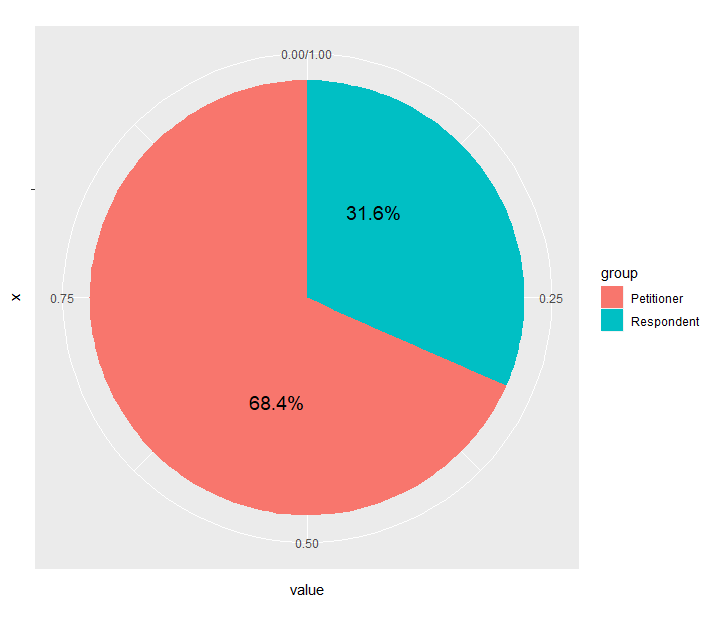
\includegraphics[width=10cm]{Piechartofcaseoutcomes.png}
\end{center}
\subsection{Table 1. Confusion Matrix for Support Vector Machine}
\begin{center}
\includegraphics[width=12cm]{"Confusion matrix for SVM".png}
\end{center}
\subsection{Table 2. Confusion Matrix for Random Forest}
\begin{center}
\includegraphics[width=12cm]{"Confusion matrix for RF".png}
\end{center}
\end{document}
